

\subsection{EXERCICE 3 (8 points)}\label{exercice-3-8-points}

\emph{Cet exercice porte sur la programmation orientée objet, sur les
arbres binaires de recherche et la récursivité.}

Chaque année, plusieurs courses de chiens de traîneaux sont organisées
sur les terrains enneigés. L'une d'elle, \emph{La Traversée Blanche},
est une course se déroulant en 9 étapes. L'organisateur de cette course
est chargé de créer un programme Python pour aider à la bonne gestion de
l'événement.

\subsubsection{Partie A : la classe
Chien}\label{partie-a-la-classe-chien}

Afin de caractériser un chien, l'organisateur décide de créer une classe
\passthrough{\lstinline!Chien!} avec les attributs suivants :

\begin{itemize}
\item
  \passthrough{\lstinline!id\_chien!}, un nombre entier correspondant au
  numéro attribué au chien lors de son inscription à la course ;
\item
  \passthrough{\lstinline!nom!}, une chaîne de caractères correspondant
  au nom du chien ;
\item
  \passthrough{\lstinline!role!}, une chaîne de caractères correspondant
  au poste occupé par le chien : en fonction de sa place dans
  l'attelage, un chien a un rôle bien défini et peut être
  \passthrough{\lstinline!'leader'!},
  \passthrough{\lstinline!'swing dog'!},
  \passthrough{\lstinline!'wheel dog'!} ou
  \passthrough{\lstinline!'team dog'!}.
\item
  \passthrough{\lstinline!id\_proprietaire!}, un nombre entier
  correspondant au numéro de l'équipe.
\end{itemize}

Le code Python incomplet de la classe \passthrough{\lstinline!Chien!}
est donné ci-dessous.

\begin{lstlisting}[language=Python]
1 class Chien:
2   def __init__(self, id_chien, nom, role, id_prop):
3       self.id_chien = id_chien
4       self.nom = nom
5       self.role = role
6       self.id_proprietaire = id_prop
7   def changer_role(self, nouveau_role):
8       """Change le rôle du chien avec la valeur passée en
            paramètre."""
9 ...
\end{lstlisting}

Voici un extrait des informations dont on dispose sur les chiens
inscrits à la course.

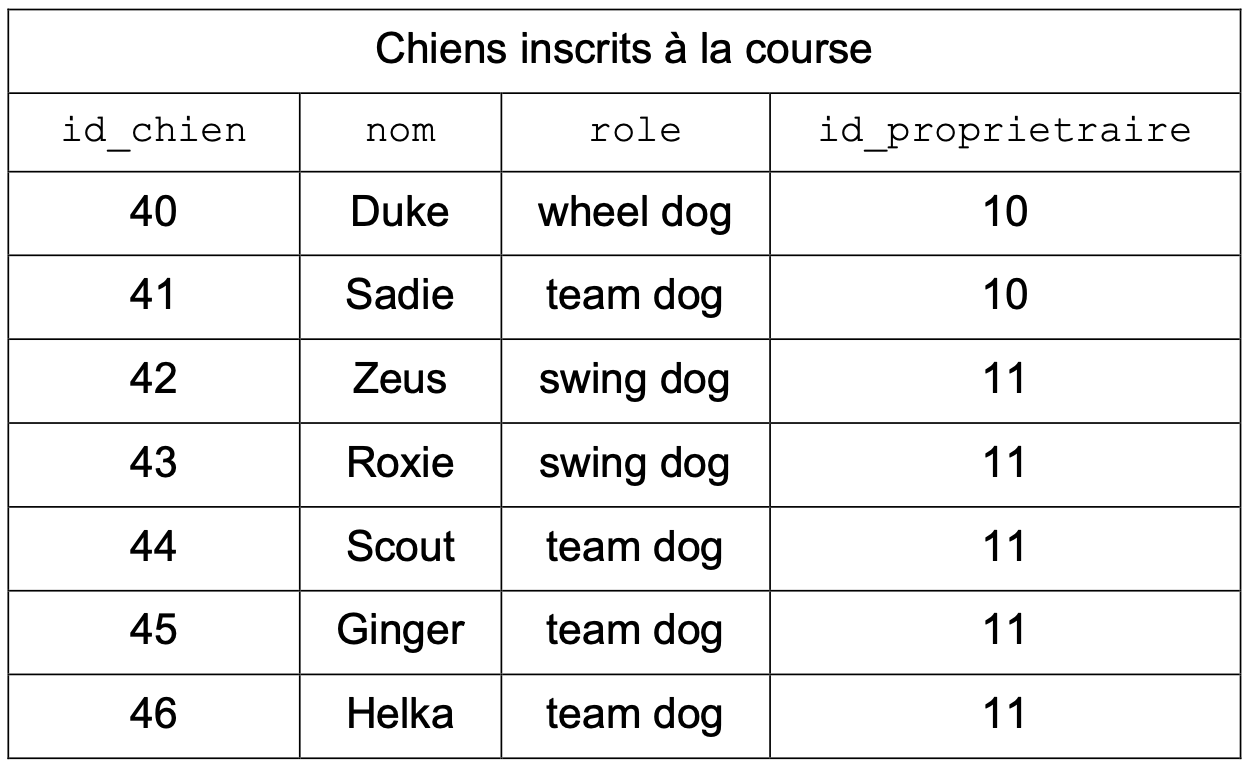
\includegraphics{24-NSIJ1ME1-Ex3-01.png}

Suite aux inscriptions, l'organisateur procède à la création de tous les
objets de type \passthrough{\lstinline!Chien!} et les stocke dans des
variables en choisissant un nom explicite. Ainsi, l'objet dont
l'attribut \passthrough{\lstinline!id\_chien!} a pour valeur 40 est
stocké dans la variable \passthrough{\lstinline!chien40!}.

\begin{enumerate}
\item
  \textbf{Écrire} l'instruction permettant d'instancier l'objet
  \passthrough{\lstinline!chien40!} caractérisant le chien ayant le
  numéro d'inscription 40.
\item
  Selon l'état de fatigue de ses chiens ou du profil de l'étape, le
  \emph{musher} (nom donné à la personne qui conduit le traîneau) peut
  décider de changer le rôle des chiens dans l'attelage.
\end{enumerate}

\textbf{Recopier} et \textbf{compléter} la méthode
\passthrough{\lstinline!changer\_role!} de la classe
\passthrough{\lstinline!Chien!}.

\begin{enumerate}
\setcounter{enumi}{2}
\item
  Le propriétaire de Duke décide de lui attribuer le rôle de
  \passthrough{\lstinline!'leader'!}.
\end{enumerate}

\textbf{Écrire} l'instruction permettant d'effectuer cette modification.

\subsubsection{Partie B : la classe
Equipe}\label{partie-b-la-classe-equipe}

On souhaite à présent créer une classe \passthrough{\lstinline!Equipe!}
ayant les attributs suivants :

\begin{itemize}
\item
  \passthrough{\lstinline!num\_dossard!}, un nombre entier correspondant
  au numéro inscrit sur le dossard du musher ;
\item
  \passthrough{\lstinline!nom\_equipe!}, une chaîne de caractères
  correspondant au nom de l'équipe ;
\item
  \passthrough{\lstinline!liste\_chiens!}, une liste d'objets de type
  \passthrough{\lstinline!Chien!} dont chaque élément correspond à un
  chien au départ de l'étape du jour ;
\item
  \passthrough{\lstinline!temps\_etape!}, une chaîne de caractères (par
  exemple \passthrough{\lstinline!'2h34'!}) représentant le temps mis
  par l'équipe pour parcourir l'étape du jour ;
\item
  \passthrough{\lstinline!liste\_temps!}, une liste de chaînes de
  caractères permettant de stocker les temps de l'équipe pour chacune
  des 9 étapes. Cet attribut peut, par exemple, contenir la liste :
  \passthrough{\lstinline!['4h36', '3h57', '3h09', '5h49', '4h45', '3h26', '4h57', '5h52', '4h31']!}.
\end{itemize}

On donne le code Python suivant de la classe
\passthrough{\lstinline!Equipe!}.

\begin{lstlisting}[language=Python]
1 class Equipe:
2   def __init__(self, num_dossard, nom_equipe):
3       self.num_dossard = num_dossard
4       self.nom_equipe = nom_equipe
5       self.liste_chiens = []
6       self.temps_etape = ''
7       self.liste_temps = []
8
9   def ajouter_chien(self, chien):
10      self.liste_chiens.append(chien)
11
12  def retirer_chien(self, numero):
13      ...
14
15  def ajouter_temps_etape(self, temps):
16      self.liste_temps.append(temps)
\end{lstlisting}

Pour la première étape, le musher de l'équipe numéro 11, représentée en
Python par l'objet \passthrough{\lstinline!eq11!}, décide de constituer
une équipe avec les quatre chiens identifiés par les numéros 42, 44, 45
et 46. On donne ci-dessous les instructions Python permettant de créer
l'équipe \passthrough{\lstinline!eq11!} et l'attelage constitué des 4
chiens précédents.

\begin{lstlisting}[language=Python]
1 eq11 = Equipe(11, 'Malamutes Endurants')
2 eq11.ajouter_chien(chien42)
3 eq11.ajouter_chien(chien44)
4 eq11.ajouter_chien(chien45)
5 eq11.ajouter_chien(chien46)
\end{lstlisting}

Malheureusement, le musher s'aperçoit que sa chienne Helka, chien numéro
46, n'est pas au mieux de sa forme et il décide de la retirer de
l'attelage.

\begin{enumerate}
\setcounter{enumi}{3}
\item
  \textbf{Recopier} et \textbf{compléter} la méthode
  \passthrough{\lstinline!retirer\_chien!} ayant pour paramètre numero,
  un entier correspondant au numéro attribué au chien lors de
  l'inscription, et permettant de mettre à jour l'attribut
  \passthrough{\lstinline!liste\_chiens!} après retrait du chien dont la
  valeur de l'attribut \passthrough{\lstinline!id\_chien!} est numero.
\item
  En vous aidant de la fonction précédente, écrire l'instruction qui
  permet de retirer Helka de l'attelage de l'équipe
  \passthrough{\lstinline!eq11!}.
\end{enumerate}

On donne à présent le code Python d'une fonction
\passthrough{\lstinline!convert!} prenant pour paramètre
\passthrough{\lstinline!chaine!}, une chaîne de caractères représentant
une durée, donnée en heure et minute.

On supposera que cette durée est toujours strictement inférieure à 10
heures, temps maximal fixé par le règlement pour terminer une étape.

\begin{lstlisting}[language=Python]
1 def convert(chaine):
2       heure_dec = int(chaine[0]) + int(chaine[2] + chaine[3])/60
3       return heure_dec
\end{lstlisting}

\begin{enumerate}
\setcounter{enumi}{5}
\item
  \textbf{Indiquer} le résultat renvoyé par l'appel
  \passthrough{\lstinline!convert('4h36')!}.
\item
  \textbf{Écrire} une fonction \passthrough{\lstinline!temps\_course!}
  qui prend pour paramètre \passthrough{\lstinline!equipe!} de type
  \passthrough{\lstinline!Equipe!} et qui renvoie un nombre flottant
  correspondant au cumul des temps de l'équipe
  \passthrough{\lstinline!equipe!} à l'issue des 9 étapes de la course.
\end{enumerate}

On rappelle que la classe \passthrough{\lstinline!Equipe!} dispose d'un
attribut \passthrough{\lstinline!liste\_temps!}.

\subsubsection{Partie C : classement à l'issue d'une
étape}\label{partie-c-classement-uxe0-lissue-dune-uxe9tape}

Chaque jour, à la fin de l'étape, on décide de construire un Arbre
Binaire de Recherche (ABR) afin d'établir le classement des équipes.
Chaque nœud de cet arbre est un objet de type
\passthrough{\lstinline!Equipe!}.

Dans cet arbre binaire de recherche, en tout nœud :

\begin{itemize}
\item
  toutes les équipes du sous-arbre gauche sont strictement plus rapides
  que ce nœud ;
\item
  toutes les équipes du sous-arbre droit sont moins rapides ou sont à
  égalité avec ce nœud.
\end{itemize}

Voici les temps, en heure et minute, relevés à l'issue de la première
étape :

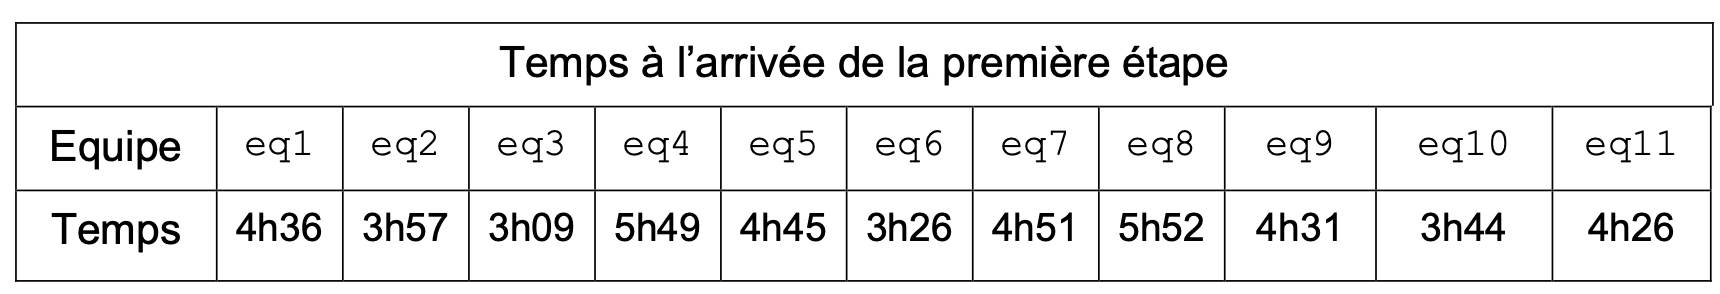
\includegraphics{24-NSIJ1ME1-Ex3-02.png}

Dans l'arbre binaire de recherche initialement vide, on ajoute
successivement, dans cet ordre, les équipes
\passthrough{\lstinline!eq1!}, \passthrough{\lstinline!eq2!},
\passthrough{\lstinline!eq3!}, \ldots, \passthrough{\lstinline!eq11!},
11 objets de la classe \passthrough{\lstinline!Equipe!} tous construits
sur le même modèle que l'objet \passthrough{\lstinline!eq11!} précédent.

\begin{enumerate}
\setcounter{enumi}{7}
\item
  Dans l'arbre binaire de recherche ci-dessous, les nœuds
  \passthrough{\lstinline!eq1!} et \passthrough{\lstinline!eq2!} ont été
  insérés.
\end{enumerate}

\textbf{Recopier} et \textbf{compléter} cet arbre en insérant les 9
nœuds manquants.

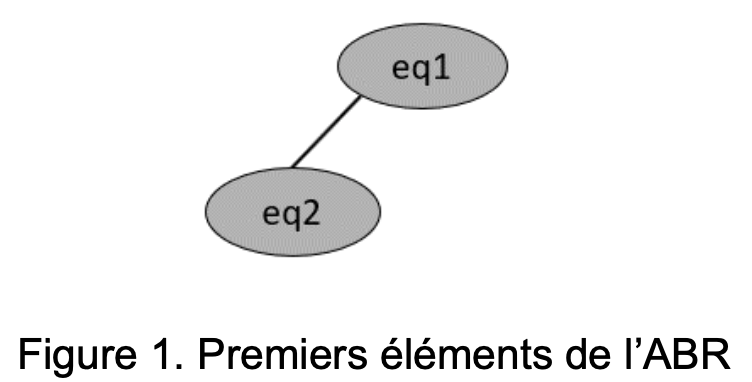
\includegraphics{24-NSIJ1ME1-Ex3-03.png}

\begin{enumerate}
\setcounter{enumi}{8}
\item
  \textbf{Indiquer} quel parcours d'arbre permet d'obtenir la liste des
  équipes classées de la plus rapide à la plus lente.
\end{enumerate}

On donne ci-dessous la classe \passthrough{\lstinline!Noeud!},
permettant de définir les arbres binaires :

\begin{lstlisting}[language=Python]
1 class Noeud:
2   def __init__(self, equipe, gauche = None, droit = None):
3       self.racine = equipe
4       self.gauche = gauche
5       self.droit = droit
\end{lstlisting}

On donne ci-dessous le code d'une fonction
\passthrough{\lstinline!construction\_arbre!} qui, à partir d'une liste
d'éléments de type \passthrough{\lstinline!Noeud!} permet d'insérer
successivement chaque nœud à sa place dans l'ABR.

\begin{lstlisting}[language=Python]
1 def construction_arbre(liste):
2   a = Noeud(liste[0])
3   for i in range(1,len(liste)):
4       inserer(a, liste[i])
5   return a
\end{lstlisting}

La fonction \passthrough{\lstinline!construction\_arbre!} fait appel à
la fonction \passthrough{\lstinline!inserer!} qui prend pour paramètre
\passthrough{\lstinline!arb!}, de type \passthrough{\lstinline!Noeud!},
et \passthrough{\lstinline!eq!}, de type
\passthrough{\lstinline!Equipe!}. Cette fonction construit le nœud à
partir de \passthrough{\lstinline!eq!} et l'insère à sa place dans
l'ABR.

\begin{lstlisting}[language=Python]
1 def inserer(arb, eq):
2   """ Insertion d'une équipe à sa place dans un ABR contenant
3   au moins un noeud."""
4   if convert(eq.temps_etape) < convert(arb.racine.temps_etape):
5       if arb.gauche is None:
6           arb.gauche = ...
7       else:
8           inserer(..., eq)
9   else:
10      if arb.droit is None:
11          arb.droit = Noeud(eq)
12      else:
13          ...
\end{lstlisting}

\begin{enumerate}
\setcounter{enumi}{9}
\item
  \textbf{Expliquer} en quoi la fonction
  \passthrough{\lstinline!inserer!} est une fonction récursive.
\item
  \textbf{Recopier} et \textbf{compléter} les lignes 6, 8 et 13 de la
  fonction \passthrough{\lstinline!inserer!}.
\item
  \textbf{Recopier} et \textbf{compléter} les lignes 3 et 5 de la
  fonction \passthrough{\lstinline!est\_gagnante!} ci-dessous qui prend
  en paramètre un ABR \passthrough{\lstinline!arbre!}, de type
  \passthrough{\lstinline!Noeud!}, et qui renvoie le nom de l'équipe
  ayant gagné l'étape.
\end{enumerate}

\begin{lstlisting}[language=Python]
1 def est_gagnante(arbre):
2     if arbre.gauche == None:
3       return ...
4     else:
5       return ...
\end{lstlisting}

\subsubsection{Partie D : classement
général}\label{partie-d-classement-guxe9nuxe9ral}

On décide d'établir un classement général obtenu à partir du cumul des
temps mis par chaque équipe pour parcourir l'ensemble des 9 étapes.

Sur le même principe que l'arbre de la partie précédente, on construit
l'ABR ci-dessous qui permet, grâce au parcours d'arbre approprié,
d'établir ce classement général des équipes.

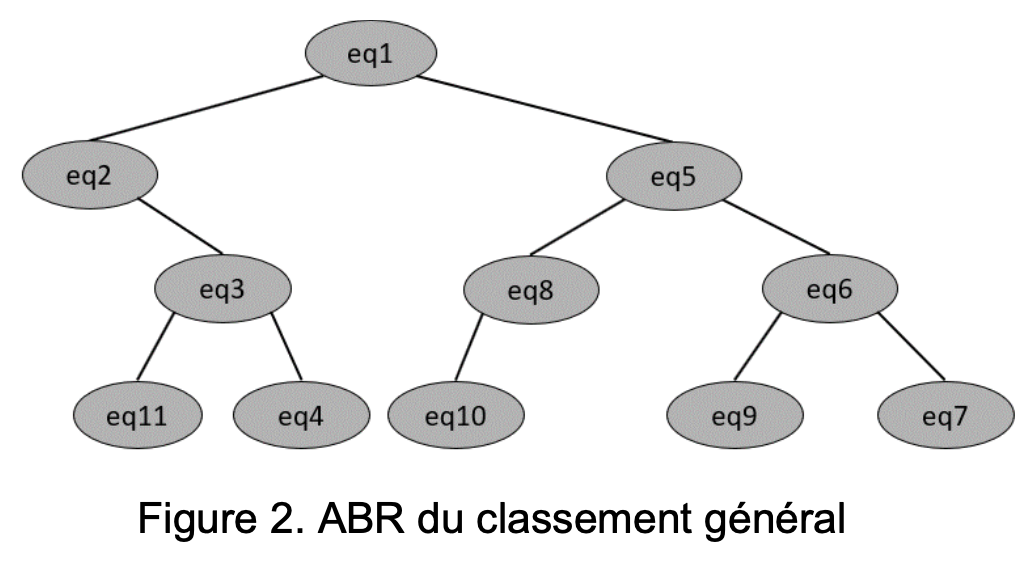
\includegraphics{24-NSIJ1ME1-Ex3-04.png}

Le règlement prévoit la disqualification d'une équipe en cas de
non-respect de celui-ci. Il s'avère que l'équipe 2 et l'équipe 5 doivent
être disqualifiées pour manquement au règlement. Les nœuds
\passthrough{\lstinline!eq2!} et \passthrough{\lstinline!eq5!} doivent
donc être supprimés de l'ABR précédent.

Pour supprimer un nœud \passthrough{\lstinline!N!} dans un ABR, trois
possibilités se présentent :

\begin{itemize}
\item
  le nœud \passthrough{\lstinline!N!} à supprimer est une feuille : il
  suffit de le retirer de l'arbre ;
\item
  le nœud \passthrough{\lstinline!N!} à supprimer n'a qu'un seul fils :
  on relie le fils de \passthrough{\lstinline!N!} au père de
  \passthrough{\lstinline!N!} et on supprime le nœud
  \passthrough{\lstinline!N!} ;
\item
  le nœud \passthrough{\lstinline!N!} à supprimer possède deux fils : on
  le remplace par son successeur (l'équipe qui a le temps immédiatement
  supérieur) qui est toujours le minimum de ses descendants droits.
\end{itemize}

\begin{enumerate}
\setcounter{enumi}{12}
\item
  Dessiner le nouvel arbre de recherche
  \passthrough{\lstinline!a\_final!} obtenu après suppression des
  équipes \passthrough{\lstinline!eq2!} et \passthrough{\lstinline!eq5!}
  dans l'ABR correspondant au classement général.
\end{enumerate}

L'organisateur souhaite disposer d'une fonction rechercher permettant de
savoir si une équipe a été disqualifiée ou non. On donne les
spécifications de la fonction \passthrough{\lstinline!rechercher!},
prenant en paramètre \passthrough{\lstinline!arbre!} et
\passthrough{\lstinline!equipe!}.

\begin{lstlisting}[language=Python]
1 def rechercher(arbre, equipe):
2   """
3       Paramètres
4       ---------
5           arbre : un ABR, non vide, de type Noeud, représentant le
6           classement général.
7           equipe : un élément, de type Equipe, dont on veut déterminer
8           l'appartenance ou non à l'ABR arbre.
9       Résultat
10      ---------
11          Cette fonction renvoie True si equipe est un nœud de arbre,
12          False sinon.
13 """
14 ...
\end{lstlisting}

Pour cette fonction (\passthrough{\lstinline!a\_final!} désigne l'arbre
obtenu à la question 13, après suppression des équipes 2 et 5) :

\begin{itemize}
\item
  l'appel \passthrough{\lstinline!rechercher(a\_final, eq1)!} renvoie
  \passthrough{\lstinline!True!} ;
\item
  l'appel \passthrough{\lstinline!rechercher(a\_final, eq2)!} renvoie
  \passthrough{\lstinline!False!}.
\end{itemize}

\begin{enumerate}
\setcounter{enumi}{13}
\item
  \textbf{Écrire} le code de la fonction
\end{enumerate}
